\chapter{Buffer Overflows}

Consideriamo il codice mostrato in Figura:
\begin{enumerate}
    \item dichiara un array di caratteri
    di 100 elementi (in C le stringhe sono rappresentate come un array di 
    caratteri, terminata da un carattere nullo); in un array di 100 caratteri possiamo
    mettere una stringa di al più 99 caratteri, perché il 100esimo sarà il 
    carattere terminatore.
    \item usa \texttt{printf} per stampare a schermo la domanda
    \item prende un input usando la funzione \texttt{scanf}: prende come primo 
    argomento una stringa che definisce in che formato vogliamo prendere l'input (ad esempio,
    \texttt{\%d} per gli interi); il secondo argomento è un puntatore all'array \texttt{name}
    \item stampa a video sostituendo al placeholder \texttt{\%s} il nome contenuto nell'array
\end{enumerate}

\begin{figure}[ht]
    \centering
    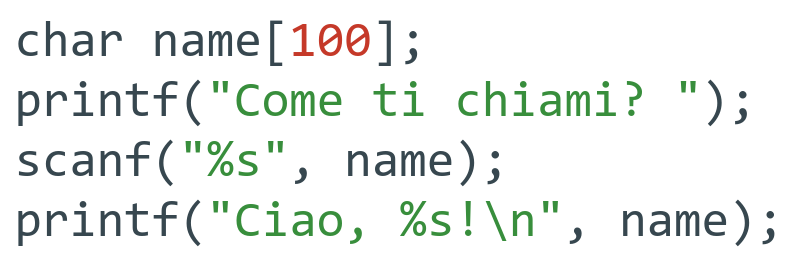
\includegraphics[width=0.5\linewidth]{images/codeex.png}
    \label{fig:ex-cprog}
\end{figure}

Questo programma è \textbf{vulnerabile} a un \textbf{buffer oveflow}: quando
prendiamo in input il nome, non c'è nessun controllo che l'utente
immetta al massimo 99 caratteri: se l'utente digita una stringa più lunga,
la parte in eccesso andrà a sovrascrivere la parte in memoria che 
segue l'array preso in considerazione, dato che C non fa nessun tipo di controllo sui \textit{bound}.

È possibile usare \texttt{scanf} in modo sicuro specificando la dimensione massima di caratteri da leggeri: ad esempio 
con \texttt{\%99s} viene specificato di legger al più 99 caratteri.


\subsubsection{Buffer overflow}
Si ha un \textbf{buffer overflow} quando il programma scrive oltre la 
fine di un buffer/array, perché ci sta copiando dentro dei dati che sono più 
grandi della dimensione del buffer.

È una delle vulnerabilità di \textbf{corruzione della memoria} classiche: stiamo scrivendo
dei dati dell'attaccate in delle locazioni di memoria che il programmatore
non aveva previsto potessero essere modificate.

\subsubsection{Conseguenze del buffer overflow}

Le garanzie di correttezza del programma \textbf{cadono completamente}. Se corrompiamo
abilmente la memoria, possiamo ottenere il \textbf{controllo completo} del processo
(poiché il processo \textit{vive} in memoria); questo caso prende il 
nome di \textit{Arbitrary code execution}, dato che posso far eseguire del 
codice arbitrario al programma che sto attaccando.

\section{Accessi out-of-bounds}
Perché nel buffer ovrlflow la funzione che \textit{prende l'input} scrive
dopo la fine dell'array?

Questo dipende dal modo in cui C fa gli accessi agli array: considerando la 
situazione in Figura, abbiamo due array uno dietro l'altro in memoria (dentro ad una \texttt{struct} 
in modo che siano sequenziali in memoria); C non fa controllo sui \textit{bound} dell'array, ma 
si limita a prendere l'indirizzo di partenza ed aggiungere l'indice moltiplicato per la dimensione 
dell'elemento.

Questo significa che accedere a \texttt{a[2]} equivale ad accedere a \texttt{b[0]}.

Accedere ad un indice fuori dai bound di un array è detto \textbf{accesso out-of-bounds}.

\begin{figure}[ht]
    \centering
    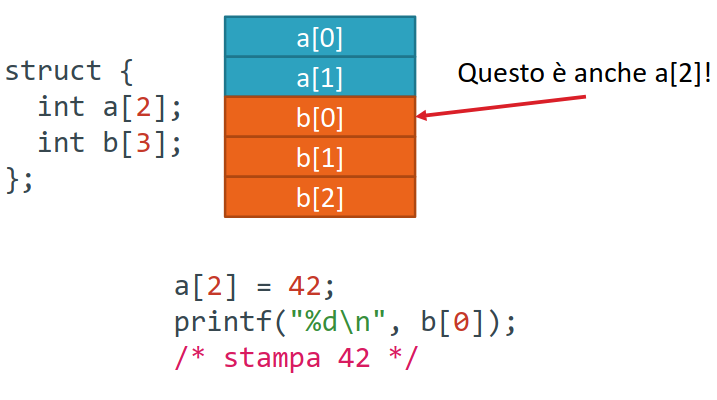
\includegraphics[width=0.75\linewidth]{images/out-bounds1.png}
    \label{fig:out-b1}
\end{figure}

\subsubsection{Un altro esempio}

Questo programma ha una \texttt{struct} con due array; chiede un indice e un valore, ed 
imposta quell'indice di \texttt{a} a quel valore. Poi stampa tutti i valori di \texttt{b}.

\begin{figure}[ht]
    \centering
    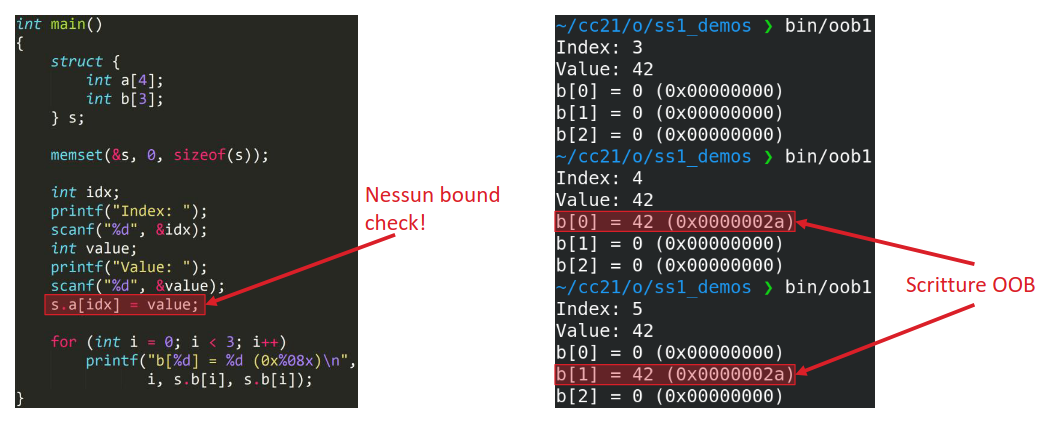
\includegraphics[width=1\linewidth]{images/out-bounds2.png}
\end{figure}

\section{Pattern pericolosi}

Vediamo in questa sezione alcuni pattern pericolosi che possono dare
origine a buffer overflows.

\begin{itemize}
    \item \textbf{senza bound checking}
    \begin{itemize}
        \item \texttt{gets} $\rightarrow$ funzione deprecata, prende come unico parametro un puntatore
        ad un array di char, da cui legge l'input; non esiste alcun modo per dire a \texttt{gets} quando fermarsi (si ferma quando trova \textit{a capo})
        \item \texttt{scanf \%s} $\rightarrow$ con \%s non verifica che la lunghezza dell'input sia minore della dimensione del buffer;
        tuttavia, è possibile usarla in modo sicuro specificando la dimensione
        \item \texttt{sprint} $\rightarrow$ scrive l'output in un buffer; se la stringa generata è più lunga del buffer c'è un overflow
        \item \texttt{strcpy} $\rightarrow$ copia la stringa da un buffer a un altro
    \end{itemize}
    \item \textbf{bound checking usato impropriamente} (la dimensione che specifico del buffer può essere 
    più grande di quella effettiva)
    \begin{itemize}
        \item \texttt{fgets}
        \item \texttt{snprintf}
        \item \texttt{strncpy}
    \end{itemize}
    \item \textbf{manipolazioni manuali}
    \begin{itemize}
        \item loop di copia
        \item accessi ad array
    \end{itemize}
\end{itemize}

\section{Un primo overflow}

Abbiamo un \textit{main} semplice che chiama la 
funzione \texttt{check\_authentication()}; se 
la funzione ritorna un valore diverso da 0 l'accesso viene consentito, altrimenti 
l'accesso è negato.

\begin{figure}[ht]
    \centering
    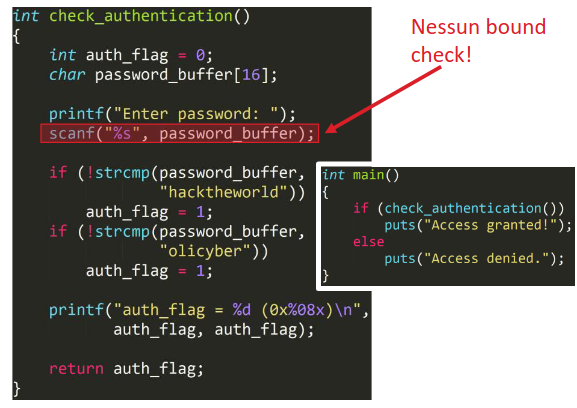
\includegraphics[width=0.75\linewidth]{images/primo-of.png}
\end{figure}

Il nostro obiettivo è ottenere l'accesso.

Il programma chiede una password e la legge in maniera insicura usando
\texttt{scanf \%s}; dopo aver letto la password la confronta con le password che conosce,
e se matcha con una di esse mette la variabile \texttt{auth\_flag = 1}; al 
termine del programma ritorna questo valore.

\subsubsection{Come possiamo fare?}
Le variabile nello stack sono disposte in ordine inverso rispetto a quello
di dichiarazione, quindi \texttt{password\_buffer} sarà prima di \texttt{auth\_flag}.

Possiamo dunque fare overflow per sovrascrivere \texttt{auth\_flag} impostandola ad un valore
diverso da 0, in modo da ottenre l'accesso.

Nell'esempio, viene fatto overflow degli ultimi due caratteri dell'input.

\begin{figure}[ht]
    \centering
    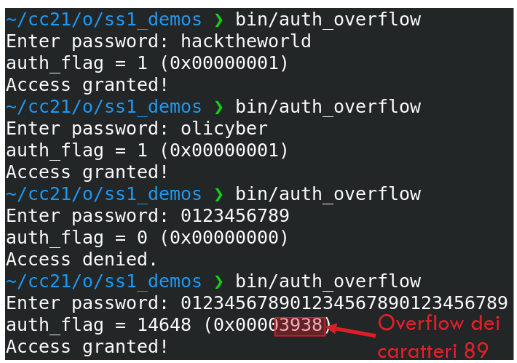
\includegraphics[width=0.75\linewidth]{images/primo-of2.png}
\end{figure}














